\documentclass[c]{beamer}



\usepackage[utf8]{inputenc}
%\usepackage[frenchb]{babel} 	% faire du fran�ais
%\usepackage{ucs}				% Accents?
\usepackage[T1]{fontenc}		% accents dans le DVI
\usepackage{geometry}
\usepackage{amsmath}
\usepackage{ragged2e}			%Texte justifi�
\usepackage{amsfonts}
%\usepackage{eurosym}			%Symbole euro
\usepackage{tikz}
\usepackage{graphicx}
\usetikzlibrary{arrows,shapes}
\usepackage{multirow}

\usepackage{setspace}
\usepackage{algorithmic,algorithm}
\renewcommand{\algorithmicrequire}{\textbf{Input:}}
\renewcommand{\algorithmicensure}{\textbf{Output:}}

%\usetheme{CambridgeUS}  %Ilmenau, CambridgeUS, Szeged, Berkeley
\usetheme{boxes}
%\useoutertheme{shadow}
\usefonttheme{serif}


\definecolor{darkgreen}{rgb}{0,0.4,0}
\def\bfm#1{\protect{\makebox{\textcolor{darkgreen}{{\boldmath $#1$}}}}}
\def\ol{\overline}              % overline (upper bound)
\def\ul{\underline}             % underline (lower bound)
\def\rounddown{{\tt rounddown}}
\def\roundup{{\tt roundup}}

\newcommand{\mult}{\cdot}
\newcommand{\Amult}{\otimes}
\newcommand{\Zf}{\mathbb{Z}[x]/\langle f \rangle}
\newcommand{\Lb}{\mathcal{L}(\textbf{B})}
\newcommand{\wn}{\omega( \sqrt{\log n})}
\newcommand{\wnd}{\omega( \sqrt{\log N})}
\newcommand{\On}{\Omega(\sqrt{n})}
\newcommand{\norm}[1]{\Vert #1 \Vert}
\newcommand{\norminf}[1]{\Vert #1 \Vert_{\infty}}
\newcommand{\normb}[1]{\Vert #1 \Vert_{2,\infty}}
\newcommand{\inner}[1]{\langle #1  \rangle}
\newcommand{\ve}[1]{\textbf{#1}}
\newcommand{\rot}[1]{\text{rot}(#1)}
\newcommand{\Rot}[1]{\text{Rot}(#1)}
\newcommand{\ps}[2]{\langle #1 , #2 \rangle}
\newcommand{\dist}{\text{dist}}
\newcommand{\mZ}{\mathbb{Z}}
\newcommand{\mQ}{\mathbb{Q}}
\newcommand{\mC}{\mathbb{C}}
\newcommand{\mR}{\mathbb{R}}
\newcommand{\mF}{\mathbb{F}}
\newcommand{\mI}{\mathcal{I}}

\newcommand{\nR}{n_{\textsc{r}}}
\newcommand{\poly}{\mathrm{poly}}
\newcommand{\eps}{\varepsilon}
\newcommand{\softOmega}{\widetilde{\Omega}}
\newcommand{\softO}{\widetilde{O}}

\newcommand{\ReRand}{\text{ReRand}}
\newcommand{\Enc}{\text{Enc}}
\newcommand{\Plain}{\text{Plain}}
\newcommand{\Ext}{\text{Ext}}
\newcommand{\MSB}{\text{MSB}}
\newcommand{\I}{\mathcal{I}}
\newcommand{\NTRU}{\textsc{ntru}}
\newcommand{\GDDH}{\textsc{gddh}}

\newcommand{\Exp}{\text{Exp}}
\newcommand{\Expb}{\overline{\text{Exp}}}
\newcommand{\samp}{\hookleftarrow}
\newcommand{\e}{\mathrm{e}}
\newcommand{\Supp}{\mathrm{Supp}}
\newcommand{\LWE}{\mathrm{LWE}}

\definecolor{MyOrange}{rgb}{1,0.49412,0.02745}
\newcommand{\MyOrange}{\color{MyOrange}}
\definecolor{MyViolet}{rgb}{0.48627,0.16471,0.60784}
\newcommand{\MyViolet}{\color{MyViolet}}
\definecolor{MyPurple}{rgb}{0.596078,0.184314,0.329412}
\newcommand{\MyPurple}{\color{MyPurple}}
\definecolor{MyGreen}{rgb}{0,0.42745,0.05098}

%% Algorithm/Experiment/Scheme references
% Algorithm: arg #1= Alg. name, arg #2= Algorithm arguments
% alg = with arguments
\newcommand{\alg}[2]{\ensuremath{\mathsf{#1}(#2)}}
% algs = with arguments and subscripts
\newcommand{\algs}[3]{\ensuremath{\mathsf{#1}_{#2}(#3)}}
% aln = no arguments
\newcommand{\aln}[1]{\ensuremath{\mathsf{#1}}}
% algsn = no arguments and subscripts
\newcommand{\algsn}[2]{\ensuremath{\mathsf{#1}_{#2}}}
% Experiment: arg#1= Experiment name, arg #2= exp arguments
% ex = with arg
\newcommand{\ex}[2]{\ensuremath{\mathbf{#1}(#2)}}
% exn = no arg
\newcommand{\exn}[1]{\ensuremath{\mathbf{#1}}}
% Scheme: arg#1= name, arg #2= arguments
% scm = with arg
\newcommand{\scm}[2]{\ensuremath{\mathsf{#1}{#2}}}
% scn = no arg
\newcommand{\scn}[1]{\ensuremath{\mathsf{#1}}}
% Table : arg#1= Table name, arg#2= table indexes (in sq. brackets)
% tabl = with arg
\newcommand{\tabl}[2]{\ensuremath{\mathsf{#1}[#2]}}
% tabn = no args
\newcommand{\tabn}[1]{\ensuremath{\mathsf{#1}}}
% Attacker Success function
% suc: arg#1 = Attacker's name, arg#2 = Scheme name, arg#3 = Notion name, arg#4 = Scheme parameters list
\newcommand{\suc}[4]{\ensuremath{\mathbf{Succ}^{\mathrm{#3}}_{#1,#2}(#4)}}
% Attacker Success function (no arguments)
% sucn: arg#1 = Attacker's name, arg#2 = Scheme name, arg#3 = Notion name
\newcommand{\sucn}[3]{\ensuremath{\mathbf{Succ}^{\mathrm{#3}}_{#1,#2}}}
% Scheme Insecurity function
% insec: arg#1 = Scheme's name, arg#2 = Notion name, arg#3 = Scheme Parameters & Attacker resource parameter list
\newcommand{\insec}[3]{\ensuremath{\mathbf{InSec}^{\mathrm{#2}}_{#1}(#3)}}
% Security Notion
%\newcommand{\snot}[1]{\ensuremath{\mathrm{#1}}}
\newcommand{\snot}[1]{#1}
%%Some of the above objects with hats (for new def.)
% algh = with arguments (and hat)
\newcommand{\algh}[2]{\ensuremath{\widehat{\mathsf{#1}}(#2)}}
% alnh = no arguments (and hat)
\newcommand{\alnh}[1]{\ensuremath{\widehat{\mathsf{#1}}}}
% ma = Modified attacker #1 with no arguments
\newcommand{\ma}[1]{\ensuremath{\widehat{\aln{#1}}}}
% uh = Applies a hat to the argument (without changing font)
\newcommand{\uh}[1]{\ensuremath{\widehat{#1}}}


%%Mathematical notation
% fdc = Function with specified name, domain and co-domain
\newcommand{\fdc}[3]{\ensuremath{#1 : #2 \rightarrow #3}}
% bis = Binary Set {0,1}
\newcommand{\bis}{\ensuremath{\{0,1\}}}
% mag = |#1|
\newcommand{\magn}[1]{\ensuremath{|#1|}}
% order = Order of argument #1 in group #2
\newcommand{\order}[2]{\ensuremath{\mathrm{Ord}_{#2}(#1)}}
% mgr = Modular group of units Z_{#1}^{*}
\newcommand{\mgr}[1]{\ensuremath{\bbbz_{#1}^{*}}}
% mrn = Modular ring Z_{#1}
\newcommand{\mrn}[1]{\ensuremath{\bbbz_{#1}}}
% defeq = Equal by Definition symbol
\newcommand{\defeq}{\ensuremath{\stackrel{\mathrm{def}}{=}}}
% inn = Inner product brackets or 'group generated by' bracket
\newcommand{\inn}[1]{\ensuremath{\langle #1 \rangle}}
% mud = Multiplication dot symbol
\newcommand{\mud}{\ensuremath{\cdot}}
% abt = Abort at step #1 event
\newcommand{\abt}[1]{\ensuremath{Ab(#1)}}
% nabt = No abort at step #1 event
\newcommand{\nabt}[1]{\ensuremath{\neg Ab(#1)}}
% supp = Support of a distribution/function
\newcommand{\supp}[1]{\ensuremath{\mathrm{Supp}(#1)}}
% sdist = Statistical distance between a pair of distributions
\newcommand{\sdist}[2]{\ensuremath{\Delta\left(#1,#2\right)}}
% flor = Floor function (largest integer not exceeding argument)
\newcommand{\flor}[1]{\ensuremath{\lfloor #1 \rfloor}}
% ceil = Ceiling function (smallest integer not less than argument)
\newcommand{\ceil}[1]{\ensuremath{\left\lceil #1 \right\rceil}}
% vc = Vector (bold math)
\newcommand{\vc}[1]{\ensuremath{\mathbf{#1}}}
% veca = Alternative vector (when bold is already used)
\newcommand{\veca}[1]{\ensuremath{\overrightarrow{#1}}}
% vecai = Alternative vector element (when bold is already used)
\newcommand{\vecai}[2]{\ensuremath{\overrightarrow{#1}[#2]}}
%% norm = Norm brackets
%\newcommand{\norm}[1]{\ensuremath{\| #1 \|}}
% lar = left arrow
\newcommand{\lar}{\ensuremath{\samp}}
% larr = leftarrow with an 'R' on top (for uniformly random selections)
\newcommand{\larr}{\ensuremath{\stackrel{\mathrm{R}}{\samp}}}
% rar = right arrow
\newcommand{\rar}{\ensuremath{\rightarrow}}
% maxo = maximum over arg. #1
\newcommand{\maxo}[1]{\ensuremath{\stackrel{\max}{#1}}}
% two case r.h.s
\newcommand{\tcrhs}[4]{\left\{ \begin{array}{ll}
                                 #1 & #2 \\
                                 #3 & #4
                                \end{array}
                         \right.}
% nat = Set of natural numbers
\newcommand{\nat}{\ensuremath{\bbbn}}
% odd = Odd part of an integer
\newcommand{\odd}[1]{\ensuremath{\mathrm{odd}(#1)}}
% lcm = Lowest Common Multiple of two integers
\newcommand{\lcm}{\ensuremath{\mathrm{lcm}}}
% xor = XOR symbol
\newcommand{\xor}{\ensuremath{\oplus}}
% rnd = Round function (Closest integer to argument)
\newcommand{\rnd}[1]{\ensuremath{\left\lceil #1 \right\rfloor}}


%%Probability stuff
% prsp = Probability Space
\newcommand{\prsp}{\ensuremath{\Sigma}}
% rv = Random variable (as a function with outcome argument)
\newcommand{\rv}[2]{\ensuremath{\mathbf{#1}(#2)}}
% rvn = Random variable (no arguments)
\newcommand{\rvn}[1]{\ensuremath{\mathbf{#1}}}
%%Some of the above objects with hats (for new def.)
% rvnh = Random variable (no arguments) with hat
\newcommand{\rvnh}[1]{\ensuremath{\widehat{\mathbf{#1}}}}
% ao = Associated outcome to the argument outcome
\newcommand{\ao}[1]{\ensuremath{\widetilde{#1}}}



%%Misc
% bol = Bold
\newcommand{\bol}[1]{\textbf{#1}}
% rom = Roman
\newcommand{\rom}[1]{\ensuremath{\mathrm{#1}}}
% tty = Typewriter
\newcommand{\tty}[1]{\ensuremath{\mathtt{#1}}}
% comm = Comment font
\newcommand{\comm}[1]{\texttt{#1}}



%%%%%%%%%%%%%%
% Algorithme %
%%%%%%%%%%%%%%



\newcounter{algorithmeligne}
%\newcommand{\instr}[1]{%\underline
%                        {\bf #1}}
%\newcommand{\nomproc}[1]{{\rm\bf #1}}
\newdimen\framewidth

\def\myframe#1{%
  \framewidth=\textwidth
  \advance\framewidth by -2pt
  \advance\framewidth by -\rightmargin
  \advance\framewidth by -\leftmargin
  \fbox{\begin{minipage}{\framewidth}#1\end{minipage}}%
}



\def\algorithme#1
{
  \setcounter{algorithmeligne}{0}
  \newcommand{\ITEM}{
    \stepcounter{algorithmeligne}
                {\footnotesize \arabic{algorithmeligne}.}
  }
  \newcommand{\lign}{\ITEM}
  \framewidth=\textwidth
  \advance\framewidth by -1pt
  \advance\framewidth by -\rightmargin
  \advance\framewidth by -\leftmargin
  \begin{center}
    \fbox{\hspace{0.08cm}\begin{minipage}{\framewidth}
        \small
        \,
        \vspace*{-.4cm}
        \begin{tabbing}
          \hskip0.5cm\=\qquad\=\qquad\=\qquad\=\qquad\=\qquad\=\qquad\=\qquad\=\qquad\=\qquad\=\qquad\\\kill
          #1
        \end{tabbing}
      \end{minipage}\hspace{0.1cm}}%
  \end{center}
  \vspace*{-.4cm}}


\setbeamercovered{transparent}


\setbeamertemplate{footline}{
\leavevmode%
\hbox{%\hspace*{-0.06cm}
\begin{beamercolorbox}[wd=.3\paperwidth,ht=2.25ex,dp=1ex,center]{section in head/foot}%
\usebeamerfont{author in head/foot}\insertshortauthor%~~(\insertshortinstitute)
\end{beamercolorbox}%
\begin{beamercolorbox}[wd=.4\paperwidth,ht=2.25ex,dp=1ex,center]{title in head/foot}%
\usebeamerfont{title in head/foot}\insertshorttitle
\end{beamercolorbox}%
\begin{beamercolorbox}[wd=.3\paperwidth,ht=2.25ex,dp=1ex,right]{section in head/foot}%
\usebeamerfont{section in head/foot}\insertshortdate{}\hspace*{2em}
\insertframenumber / \inserttotalframenumber\hspace*{2ex}
\end{beamercolorbox}}%
\vskip0pt%
}

%\newcommand{\mult}{\mathop{.}}
%\newcommand{\Zf}{\mathbb{Z}[x]/\langle f \rangle}
%\newcommand{\Lb}{\mathcal{L}(\textbf{B})}
%\newcommand{\wn}{\omega( \sqrt{\log n})}
%\newcommand{\norm}[1]{\Vert #1 \Vert}
%\newcommand{\ve}[1]{\textbf{#1}}
%\newcommand{\rot}[1]{\text{rot}(#1)}
%\newcommand{\Rot}[1]{\text{Rot}(#1)}
%\newcommand{\preuve}{\noindent \textit{Preuve.} }
%\newcommand{\softOmega}{\widetilde{\Omega}}
%\newcommand{\cqfd}{\begin{flushright} $\square$  \end{flushright}}

%\AtBeginSection[]
%{
%\begin{frame}<beamer>
%\frametitle{\textcolor{white}{Plan}}
%\tableofcontents[currentsection]
%\end{frame}
%}

\title[JDD]{Journée des doctorants}

\newcommand{\absent}{\textcolor{gray}}
\author[AriC]{ {Silviu Filip}
  \and {Sébastien Maulat}
  \and {\absent{Stephen Melczer}} \\
  \and {Vincent Neiger}
  \and {\absent{Marie Paindavoine}} \\
  \and {Antoine Plet}
  \and {\absent{Valentina Popescu}} }

\institute{Aric Team, LIP, ENS de Lyon, France}
  
\date{June 2015}

 %\date{4th of december 2012}
\begin{document}

\setbeamertemplate{navigation symbols}{}
% For every picture that defines or uses external nodes, you'll have to
% apply the 'remember picture' style. To avoid some typing, we'll apply
% the style to all pictures.
\tikzstyle{every picture}+=[remember picture]

% By default all math in TikZ nodes are set in inline mode. Change this to
% displaystyle so that we don't get small fractions.
%\everymath{\displaystyle}

\begin{frame}
 \titlepage
 % \begin{flushright}
%\includegraphics[width=1.6cm]{ERC-logo.png}
%\end{flushright}
 
\end{frame}

%%/begin AERES slides
\begin{frame}
\frametitle{AriC: Arithmetic and Computing}
Améliorer le \alert{calcul}, en termes de \alert{performance, d'efficacité} et de \alert{fiabilité.}
\break
\begin{center}
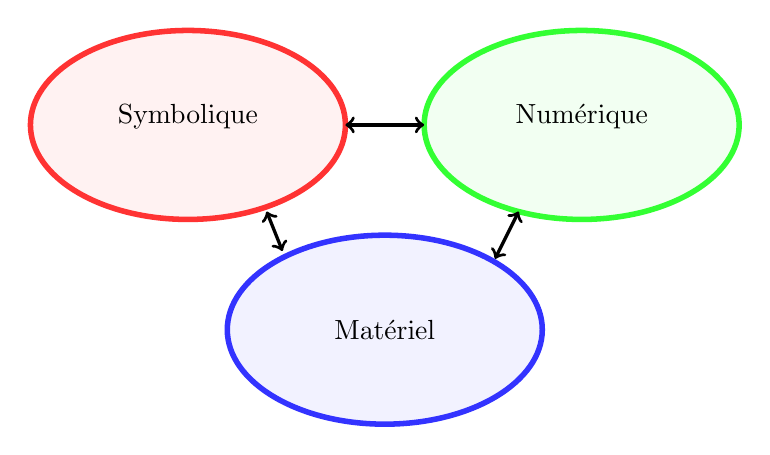
\begin{tikzpicture}[scale=0.1]
\fill[red!05] (0,1) ellipse (20 and 12);
\draw[red!80, line width = 2] (0,1) ellipse (20 and 12);
\draw(0,2) node{Symbolique};
\fill[green!05] (50,1) ellipse (20 and 12);
\draw[green!80, line width = 2] (50,1) ellipse (20 and 12);
\draw(50,2) node{Numérique};
\draw[very thick,<->] (20,1) -- (30,1);
\fill[blue!05] (25,-25) ellipse (20 and 12);
\draw[blue!80, line width = 2] (25,-25) ellipse (20 and 12);
\draw(25,-25) node{Matériel};
\draw[very thick,<->] (10,-10) -- (12,-15);
\draw[very thick,<->] (39,-16) -- (42,-10);
\end{tikzpicture}
\end{center}

\end{frame}


\begin{frame}
\frametitle{AriC: Arithmetic and Computing}
%Améliorer le \alert{calcul}, en termes de \alert{performance, d'efficacité} et de \alert{fiabilité.}
\begin{itemize}
\item algorithmes arithmétiques $\&$ implantation:\\ %(matérielle, logicielle): \\
  \begin{minipage}{7cm}  
    \begin{itemize}
    \item %arithmétique entière et
      virgule flottante;
    \item %arithmétique complexe,
      multi-précision;
    \item bornes d'erreur fines
      \end{itemize} \end{minipage}~~
      \begin{minipage}{3cm}
      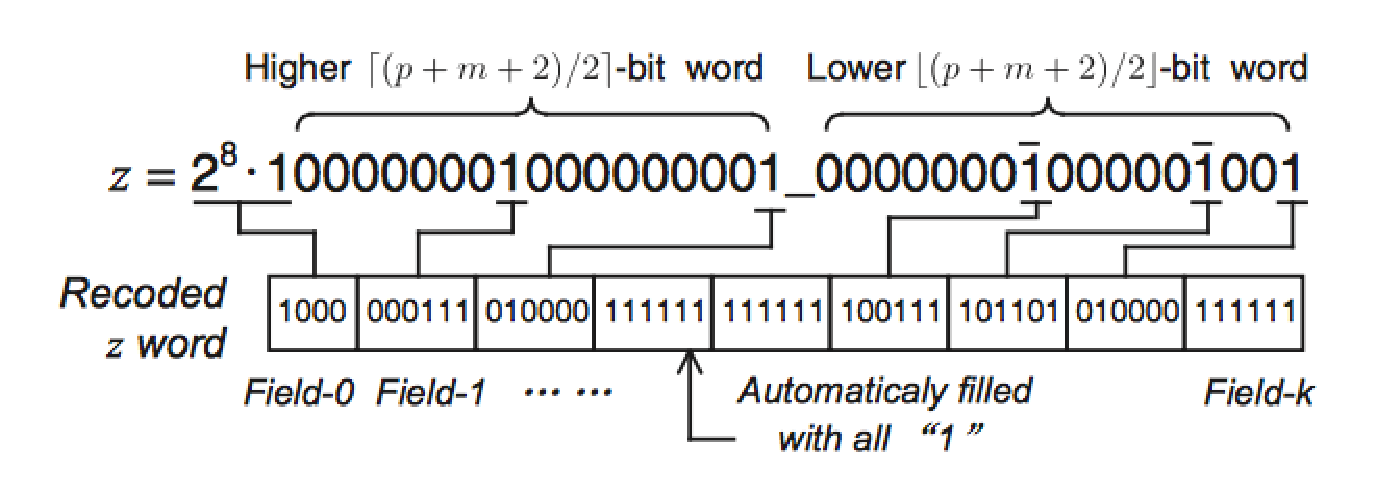
\includegraphics[width=2.9cm]{VisiteAERES2014/Figures/archisin.pdf}
    \end{minipage}

    \item méthodes d'approximation: \\
    \begin{minipage}{6.9cm}
      \begin{itemize}
            \item uniforme/ponctuelle;
%            \item certifiée;
            \item polynomiale/rationnelle
       \end{itemize}
         \end{minipage}~~~~
      \begin{minipage}{3cm}
      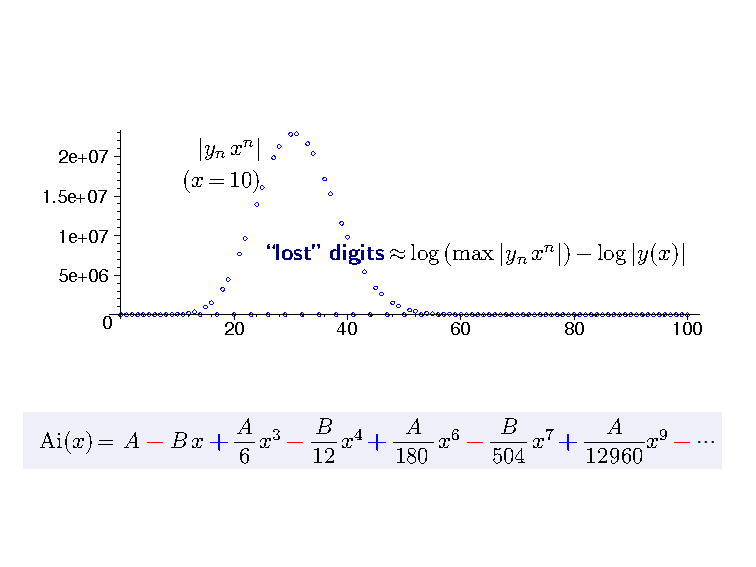
\includegraphics[width=2.5cm]{VisiteAERES2014/Figures/mezzarobba-arith.pdf}
       \end{minipage}
    % \item  réseaux euclidiens et cryptographie:\\[-0.2cm]
    % \begin{minipage}{6.9cm}
    %    \begin{itemize}
    %         \item algorithmique des réseaux;
    %         \item cryptographie reposant sur les réseaux;
    %     \end{itemize}
    %   \end{minipage}~~~~
    %   \begin{minipage}{3cm}
    %   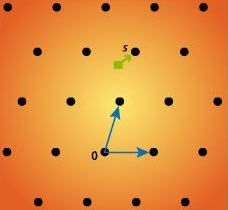
\includegraphics[width=1.6cm]{VisiteAERES2014/Figures/Resau.jpg}
    %   \end{minipage}
     \item calcul certifié et calcul formel:\\
       \vskip .5em
      \begin{minipage}{10cm}
        \begin{itemize}
       \item algèbre linéaire à coefficients polynomiaux;
       \item récurrences linéaires à coefficients polynomiaux;
%       \item arithmétique d'intervalles.
    \end{itemize}
  \end{minipage}
\end{itemize}
\end{frame}
%%/end AERES slides

\begin{frame}<1>
  \frametitle{\textcolor{red}{AriC}}

  \tikzstyle{na} = [baseline=-.5ex]

  \begin{columns}
    \begin{column}{0.18\textwidth}
      \hspace*{-.7cm}\tikz[baseline]{
        \node[fill=red!10,anchor=base,text width=2.6cm, text centered]
        (n1) {\begin{tiny}
            \textbf{Exact}
            \hspace{1.5cm}
            Exact arithmetic
            \hspace{0.5cm}
            Computer algebra
            \hspace{2.2cm}
            \textbf{Approximate}
            \hspace{0.5cm}
            Floating-point arithmetic
            \hspace{1cm}
            Interval arithmetic
        \end{tiny}};}
    \end{column}

    \begin{column}{0.08\textwidth}
      \uncover<1-3>{\hspace*{-1cm}\tikz[baseline]{ \node[fill=white!30,anchor=base,text width=3cm, text centered,scale=1] (t1) {\color{red} {\footnotesize  Structured linear algebra } };}}

      \vspace{2cm}

      \uncover<1-4>{\tikz[baseline]{ \node[anchor=base, text centered,scale=1] (t2) {\color{red}{\footnotesize Lattices }}; }}


      \vspace{2cm}

      \uncover<1,4,5>{\hspace*{-1cm}\tikz[baseline]{ \node[fill=white!20,anchor=base,text width=2.8cm, text centered,scale=1] (t3) {\color{red}  {\footnotesize Numerical Linear Algebra}} ; }}

    \end{column}


    \column{0.2\textwidth}

    \uncover<1,2>{\hspace*{-1.2cm}\tikz[baseline]{\node[anchor=base,text width=1.5cm, text centered,scale=1] (t4) {\color{red} \begin{tiny}
          Polynomial
      \end{tiny}};}}

    \vspace*{0.1cm}

    \uncover<1,3,4>{\hspace*{-1.2cm}\tikz[baseline]{\node[ellipse,anchor=base,text width=1cm, text centered,scale=1] (t5) {\color{red} {\tiny Euclidean}};}}



    \column{0.3\textwidth}
    \uncover<1,2>{\hspace*{-1.5cm}\tikz[baseline]{\node[fill=white!30,anchor=base,text width=2cm, text centered,scale=1] (n2) {{\footnotesize Multivariate Interpolation }};}}

    \vspace*{1cm}

    \uncover<1,3>{\hspace*{-1.5cm}\tikz[baseline]{\node[fill=white!20,anchor=base,text width=3.5cm, text centered,scale=1] (n3) {{\footnotesize Learning With Errors structured version }};}}

    \vspace*{1.2cm}

    \uncover<1,4>{\hspace*{-1.5cm}\tikz[baseline]{\node[fill=white!20,anchor=base,text width=3cm, text centered,scale=1] (n4) {{\footnotesize Numerical functions and digital filters}};}}

    \vspace*{1cm}

    \uncover<1,5>{\hspace*{-1.5cm}\tikz[baseline]{\node[fill=white!20,anchor=base,text width=2.5cm, text centered,scale=1] (n5) {{\footnotesize Interval Linear Algebra}};}}
    %\end{column}



    \column{0.1\textwidth}
    \uncover<1,2>{\hspace*{-1.5cm}\tikz[baseline]{\node[fill=white!20,anchor=base,text width=3cm, text centered,scale=1] (m2) {{\scriptsize Applications to error-correcting codes}};}}

    \vspace*{1cm}

    \uncover<1,3>{\hspace*{-1.2cm}\tikz[baseline]{\node[fill=white!20,anchor=base,text width=2cm, text centered,scale=1] (m3) {{\scriptsize Cryptographic applications}};}}

    \vspace*{1cm}

    \uncover<1,4>{\hspace*{-1.5cm}\tikz[baseline]{\node[fill=white!20,anchor=base,text width=3cm, text centered,scale=1] (m4) {{\scriptsize FPGA Implementations}};}}

    \vspace*{1cm}

    \uncover<1,5>{\hspace*{-1.5cm}\tikz[baseline]{\node[fill=white!20,anchor=base,text width=3cm, text centered,scale=1] (m5) {{\scriptsize Certified parallel linear algebra library}};}}


  \end{columns}

  \begin{tikzpicture}[overlay]
    \uncover<1-3>{\path[black, thick,->] (n1) edge [out=80, in=180] (t1);}
    \uncover<1-4>{\path[black,thick,->] (n1) edge [out=0, in=180] (t2);}
    \uncover<1,4,5>{\path[black,thick,->] (n1) edge [out=-80, in=180] (t3);}
    \uncover<1,3>{\path[red!40,thick,->] (t5) edge [out=5, in=185] (n3);}
    \uncover<1,2>{\path[MyGreen!40,thick,->] (t4) edge [out=25, in=210] (n2);}
    \uncover<1,4>{\path[blue!50,thick,->] (t5) edge [out=0, in=175] (n4);}
    \uncover<1,4>{\path[blue!50,thick,->] (t3) edge [out=10, in=185] (n4);}
    \uncover<1,5>{\path[MyPurple!70,thick,->] (t3) edge [out=-5, in=175] (n5);}
    \uncover<1,2>{\path[MyGreen!40,thick,->] (t1) edge [out=5, in=190] (n2);}
    \uncover<1,3>{\path[red!40,thick,->] (t1) edge [out=-5, in=175] (n3);}
    \uncover<1,2>{\path[MyGreen!50,thick,->] (n2) edge [out=0, in=180] (m2);}
    \uncover<1,3>{\path[red!40,thick,->] (n3) edge [out=-10, in=180] (m3);}
    \uncover<1,4>{\path[blue!50,thick,->] (n4) edge [out=0, in=180] (m4);}
    \uncover<1,5>{\path[MyPurple!70,thick,->] (n5) edge [out=0, in=180] (m5);}
    
    
  \end{tikzpicture}
\end{frame}



%
%\begin{frame}
%\frametitle{Outline}
%
%\tableofcontents
%
%\end{frame}


%
% Vincent's part
%

\begin{frame}<2>
  \frametitle{\textcolor{red}{AriC}}

  \tikzstyle{na} = [baseline=-.5ex]

  \begin{columns}
    \begin{column}{0.18\textwidth}
      \hspace*{-.7cm}\tikz[baseline]{
        \node[fill=red!10,anchor=base,text width=2.6cm, text centered]
        (n1) {\begin{tiny}
            \textbf{Exact}
            \hspace{1.5cm}
            Exact arithmetic
            \hspace{0.5cm}
            Computer algebra
            \hspace{2.2cm}
            \textbf{Approximate}
            \hspace{0.5cm}
            Floating-point arithmetic
            \hspace{1cm}
            Interval arithmetic
        \end{tiny}};}
    \end{column}

    \begin{column}{0.08\textwidth}
      \uncover<1-3>{\hspace*{-1cm}\tikz[baseline]{ \node[fill=white!30,anchor=base,text width=3cm, text centered,scale=1] (t1) {\color{red} {\footnotesize  Structured linear algebra } };}}

      \vspace{2cm}

      \uncover<1-4>{\tikz[baseline]{ \node[anchor=base, text centered,scale=1] (t2) {\color{red}{\footnotesize Lattices }}; }}


      \vspace{2cm}

      \uncover<1,4,5>{\hspace*{-1cm}\tikz[baseline]{ \node[fill=white!20,anchor=base,text width=2.8cm, text centered,scale=1] (t3) {\color{red}  {\footnotesize Numerical Linear Algebra}} ; }}

    \end{column}


    \column{0.2\textwidth}

    \uncover<1,2>{\hspace*{-1.2cm}\tikz[baseline]{\node[anchor=base,text width=1.5cm, text centered,scale=1] (t4) {\color{red} \begin{tiny}
          Polynomial
      \end{tiny}};}}

    \vspace*{0.1cm}

    \uncover<1,3,4>{\hspace*{-1.2cm}\tikz[baseline]{\node[ellipse,anchor=base,text width=1cm, text centered,scale=1] (t5) {\color{red} {\tiny Euclidean}};}}



    \column{0.3\textwidth}
    \uncover<1,2>{\hspace*{-1.5cm}\tikz[baseline]{\node[fill=white!30,anchor=base,text width=2cm, text centered,scale=1] (n2) {{\footnotesize Multivariate Interpolation}};}}

    \vspace*{1cm}

    \uncover<1,3>{\hspace*{-1.5cm}\tikz[baseline]{\node[fill=white!20,anchor=base,text width=3.5cm, text centered,scale=1] (n3) {{\footnotesize Learning With Errors structured version }};}}

    \vspace*{1.2cm}

    \uncover<1,4>{\hspace*{-1.5cm}\tikz[baseline]{\node[fill=white!20,anchor=base,text width=3cm, text centered,scale=1] (n4) {{\footnotesize Numerical functions and digital filters}};}}

    \vspace*{1cm}

    \uncover<1,5>{\hspace*{-1.5cm}\tikz[baseline]{\node[fill=white!20,anchor=base,text width=2.5cm, text centered,scale=1] (n5) {{\footnotesize Interval Linear Algebra}};}}
    %\end{column}



    \column{0.1\textwidth}
    \uncover<1,2>{\hspace*{-1.5cm}\tikz[baseline]{\node[fill=white!20,anchor=base,text width=3cm, text centered,scale=1] (m2) {{\scriptsize Applications to error-correcting codes}};}}

    \vspace*{1cm}

    \uncover<1,3>{\hspace*{-1.2cm}\tikz[baseline]{\node[fill=white!20,anchor=base,text width=2.5cm, text centered,scale=1] (m3) {{\scriptsize Cryptographic applications}};}}

    \vspace*{1cm}

    \uncover<1,4>{\hspace*{-1.5cm}\tikz[baseline]{\node[fill=white!20,anchor=base,text width=3cm, text centered,scale=1] (m4) {{\scriptsize FPGA Implementations}};}}

    \vspace*{1cm}

    \uncover<1,5>{\hspace*{-1.5cm}\tikz[baseline]{\node[fill=white!20,anchor=base,text width=3cm, text centered,scale=1] (m5) {{\scriptsize Certified parallel linear algebra library}};}}


  \end{columns}

  \begin{tikzpicture}[overlay]
    \uncover<1-3>{\path[black, thick,->] (n1) edge [out=80, in=180] (t1);}
    \uncover<1-4>{\path[black,thick,->] (n1) edge [out=0, in=180] (t2);}
    \uncover<1,4,5>{\path[black,thick,->] (n1) edge [out=-80, in=180] (t3);}
    \uncover<1,3>{\path[red!40,thick,->] (t5) edge [out=5, in=185] (n3);}
    \uncover<1,2>{\path[MyGreen!40,thick,->] (t4) edge [out=25, in=210] (n2);}
    \uncover<1,4>{\path[blue!50,thick,->] (t5) edge [out=0, in=175] (n4);}
    \uncover<1,4>{\path[blue!50,thick,->] (t3) edge [out=10, in=185] (n4);}
    \uncover<1,5>{\path[MyPurple!70,thick,->] (t3) edge [out=-5, in=175] (n5);}
    \uncover<1,2>{\path[MyGreen!40,thick,->] (t1) edge [out=5, in=190] (n2);}
    \uncover<1,3>{\path[red!40,thick,->] (t1) edge [out=-5, in=175] (n3);}
    \uncover<1,2>{\path[MyGreen!50,thick,->] (n2) edge [out=0, in=180] (m2);}
    \uncover<1,3>{\path[red!40,thick,->] (n3) edge [out=0, in=180] (m3);}
    \uncover<1,4>{\path[blue!50,thick,->] (n4) edge [out=0, in=180] (m4);}
    \uncover<1,5>{\path[MyPurple!70,thick,->] (n5) edge [out=0, in=180] (m5);}
    
    
  \end{tikzpicture}
\end{frame}


\begin{frame}
	\frametitle{\textcolor{red}{AriC} --- Multivariate interpolation}

	Problem: \structure{\textsc{multivariate polynomial interpolation}}

	\bigskip
	Applications to:
	\begin{itemize}
		\item \alert{Error-correcting codes}\\
			Enable \structure{reliable} delivery of data over 
	\structure{unreliable} communication channels \\
	(add \structure{redundancy} to the message)
	\item \alert{Crypto: private information retrieval} \\
		look up information in an \structure{online database} \alert{without} 
		\alert{letting the database servers} \structure{know (or learn)} 
		the query terms or responses.
	\end{itemize}
\end{frame}

\begin{frame}
	\frametitle{\textcolor{red}{AriC} --- Tool: structured matrices}

	Find a \alert{solution} of a (scalar) \alert{structured linear system},
	\begin{figure}
		\centering
		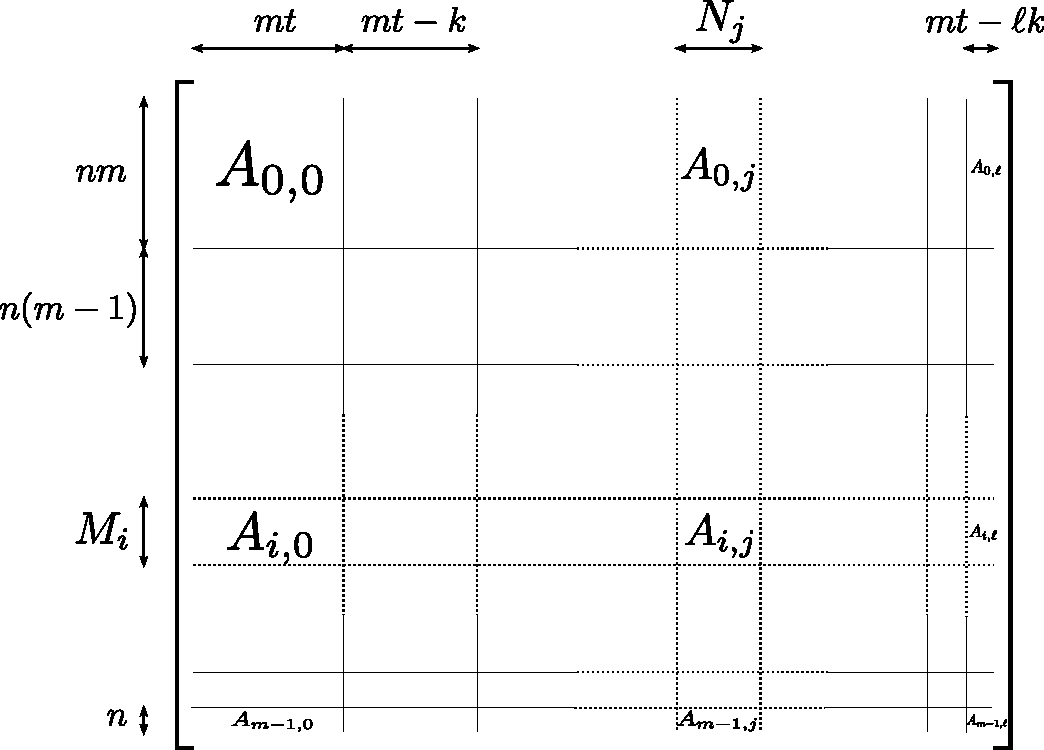
\includegraphics[width=0.8\textwidth]{JDD2014/figures/block_hankel_system.pdf}
	\end{figure}
	where $A_{i,j}$ is a \structure{Toeplitz} / \structure{Hankel} 
	/ \structure{Vandermonde} / \ldots{} matrix
\end{frame}

\begin{frame}
	\frametitle{\textcolor{red}{AriC} --- Tool: polynomial matrices}

	Find a \alert{short vector} in the row space of a \alert{polynomial matrix}\\
	$=$ \structure{lattice basis reduction} (LLL), over the polynomials

	\medskip
	Example matrix (for list-decoding Reed-Solomon codes):
	\begin{figure}
		\centering
		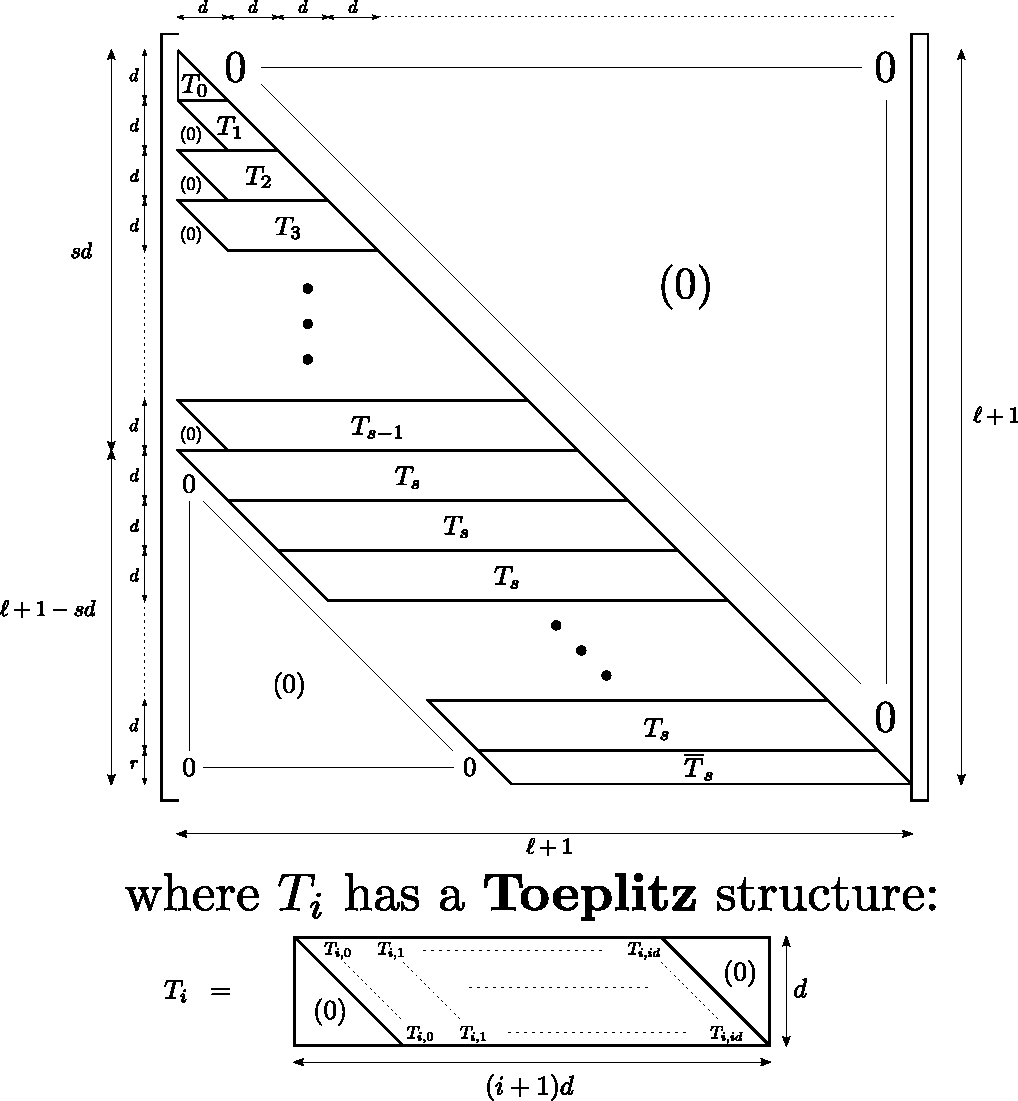
\includegraphics[width=0.55\textwidth]{JDD2014/figures/structured_lattice_matrix.pdf}
	\end{figure}
\end{frame}

%
% Partie Adeline
%

\begin{frame}<3>
  \frametitle{\textcolor{red}{AriC}}

  \tikzstyle{na} = [baseline=-.5ex]

  \begin{columns}
    \begin{column}{0.18\textwidth}
      \hspace*{-.7cm}\tikz[baseline]{
        \node[fill=red!10,anchor=base,text width=2.6cm, text centered]
        (n1) {\begin{tiny}
            \textbf{Exact}
            \hspace{1.5cm}
            Exact arithmetic
            \hspace{0.5cm}
            Computer algebra
            \hspace{2.2cm}
            \textbf{Approximate}
            \hspace{0.5cm}
            Floating-point arithmetic
            \hspace{1cm}
            Interval arithmetic
        \end{tiny}};}
    \end{column}

    \begin{column}{0.08\textwidth}
      \uncover<1-3>{\hspace*{-1cm}\tikz[baseline]{ \node[fill=white!30,anchor=base,text width=3cm, text centered,scale=1] (t1) {\color{red} {\footnotesize  Structured linear algebra } };}}

      \vspace{2cm}

      \uncover<1-4>{\tikz[baseline]{ \node[anchor=base, text centered,scale=1] (t2) {\color{red}{\footnotesize Lattices }}; }}


      \vspace{2cm}

      \uncover<1,4,5>{\hspace*{-1cm}\tikz[baseline]{ \node[fill=white!20,anchor=base,text width=2.8cm, text centered,scale=1] (t3) {\color{red}  {\footnotesize Numerical Linear Algebra}} ; }}

    \end{column}


    \column{0.2\textwidth}

    \uncover<1,2>{\hspace*{-1.2cm}\tikz[baseline]{\node[anchor=base,text width=1.5cm, text centered,scale=1] (t4) {\color{red} \begin{tiny}
          Polynomial
      \end{tiny}};}}

    \vspace*{0.1cm}

    \uncover<1,3,4>{\hspace*{-1.2cm}\tikz[baseline]{\node[ellipse,anchor=base,text width=1cm, text centered,scale=1] (t5) {\color{red} {\tiny Euclidean}};}}



    \column{0.3\textwidth}
    \uncover<1,2>{\hspace*{-1.5cm}\tikz[baseline]{\node[fill=white!30,anchor=base,text width=2cm, text centered,scale=1] (n2) {{\footnotesize Multivariate Interpolation}};}}

    \vspace*{1cm}

    \uncover<1,3>{\hspace*{-1.5cm}\tikz[baseline]{\node[fill=white!20,anchor=base,text width=3.5cm, text centered,scale=1] (n3) {{\footnotesize Learning With Errors structured version }};}}

    \vspace*{1.2cm}

    \uncover<1,4>{\hspace*{-1.5cm}\tikz[baseline]{\node[fill=white!20,anchor=base,text width=3cm, text centered,scale=1] (n4) {{\footnotesize Numerical functions and digital filters}};}}

    \vspace*{1cm}

    \uncover<1,5>{\hspace*{-1.5cm}\tikz[baseline]{\node[fill=white!20,anchor=base,text width=2.5cm, text centered,scale=1] (n5) {{\footnotesize Interval Linear Algebra}};}}
    %\end{column}



    \column{0.1\textwidth}
    \uncover<1,2>{\hspace*{-1.5cm}\tikz[baseline]{\node[fill=white!20,anchor=base,text width=3cm, text centered,scale=1] (m2) {{\scriptsize Applications to error-correcting codes}};}}

    \vspace*{1cm}

    \uncover<1,3>{\hspace*{-1.2cm}\tikz[baseline]{\node[fill=white!20,anchor=base,text width=2.5cm, text centered,scale=1] (m3) {{\scriptsize Cryptographic applications}};}}

    \vspace*{1cm}

    \uncover<1,4>{\hspace*{-1.5cm}\tikz[baseline]{\node[fill=white!20,anchor=base,text width=3cm, text centered,scale=1] (m4) {{\scriptsize FPGA Implementations}};}}

    \vspace*{1cm}

    \uncover<1,5>{\hspace*{-1.5cm}\tikz[baseline]{\node[fill=white!20,anchor=base,text width=3cm, text centered,scale=1] (m5) {{\scriptsize Certified parallel linear algebra library}};}}


  \end{columns}

  \begin{tikzpicture}[overlay]
    \uncover<1-3>{\path[black, thick,->] (n1) edge [out=80, in=180] (t1);}
    \uncover<1-4>{\path[black,thick,->] (n1) edge [out=0, in=180] (t2);}
    \uncover<1,4,5>{\path[black,thick,->] (n1) edge [out=-80, in=180] (t3);}
    \uncover<1,3>{\path[red!40,thick,->] (t5) edge [out=5, in=185] (n3);}
    \uncover<1,2>{\path[MyGreen!40,thick,->] (t4) edge [out=25, in=210] (n2);}
    \uncover<1,4>{\path[blue!50,thick,->] (t5) edge [out=0, in=175] (n4);}
    \uncover<1,4>{\path[blue!50,thick,->] (t3) edge [out=10, in=185] (n4);}
    \uncover<1,5>{\path[MyPurple!70,thick,->] (t3) edge [out=-5, in=175] (n5);}
    \uncover<1,2>{\path[MyGreen!40,thick,->] (t1) edge [out=5, in=190] (n2);}
    \uncover<1,3>{\path[red!40,thick,->] (t1) edge [out=-5, in=175] (n3);}
    \uncover<1,2>{\path[MyGreen!50,thick,->] (n2) edge [out=0, in=180] (m2);}
    \uncover<1,3>{\path[red!40,thick,->] (n3) edge [out=0, in=180] (m3);}
    \uncover<1,4>{\path[blue!50,thick,->] (n4) edge [out=0, in=180] (m4);}
    \uncover<1,5>{\path[MyPurple!70,thick,->] (n5) edge [out=0, in=180] (m5);}
    
    
  \end{tikzpicture}
\end{frame}




\begin{frame}
\frametitle{\textcolor{red}{AriC} -- Lattice-Based Cryptography}

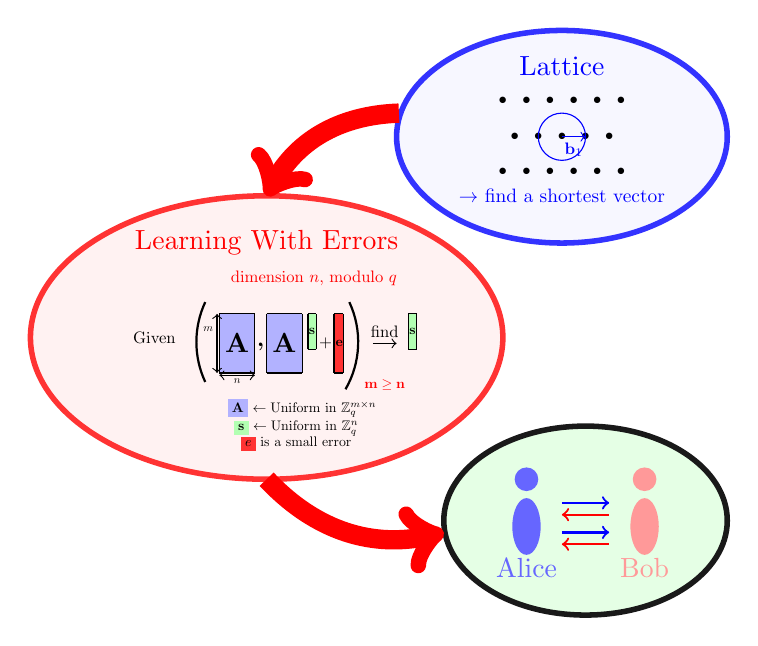
\begin{tikzpicture}[scale=0.15]
\fill[red!05] (0,1) ellipse (20 and 12);
\draw[red!80, line width = 2] (0,1) ellipse (20 and 12);
\draw (0,9) node[red,scale=1] {Learning With Errors};
\draw (4,6) node[red, scale=0.6] {dimension $n$, modulo $q$};
\draw (3,-5) node[scale=0.5]  {\colorbox{blue!30}{$\mathbf{A}$} $\leftarrow \text{Uniform in }\mathbb{Z}_q^{m \times n}$};
\draw (2.5,-6.7) node[scale=0.5]  {\colorbox{green!30}{$\mathbf{s}$} $\leftarrow \text{Uniform in } \mathbb{Z}_q^{n}$};
\draw (2.5,-8) node[scale=0.5]  { \colorbox{red!80}{$e$} is a small error};
\draw (10,-3) node[red,scale=0.5]  { $ \mathbf{ m \geq n }$ };

\draw[thick] (-5.2,4) arc (155:205:8) ;
\draw[thick] (7,4) arc (25:-30:8) ;

\draw (-0.5,0.2) node[scale=0.8] {\textbf{,}};
\draw [->] (9,0.5) -- (11,0.5) node[scale=0.6] [midway, above] {find};
\fill[green!30] (12,0) rectangle (12.7,3) ;
\draw (12,0) -- (12,3) ;
\draw (12,0) -- (12.7,0) ;
\draw (12,3) -- (12.7,3) ;
\draw (12.7,0) -- (12.7,3) ;
\draw (12.35,1.5) node[scale=0.5] {$ \mathbf{s} $};

\draw (-9.5,1) node[scale=0.6] {Given};

\fill[blue!30] (-4,-2) rectangle (-1,3) ;
\draw (-4,-2) -- (-4,3) ;
\draw (-1,-2) -- (-1,3) ;
\draw (-4,-2) -- (-1,-2) ;
\draw (-4,3) -- (-1,3) ;
\draw (-2.5,0.5) node[scale=1] {$\mathbf{A}$} ;

% Matrice 1
\fill[blue!30] (0,-2) rectangle (3,3) ;
\draw (0,-2) -- (0,3) ;
\draw (3,-2) -- (3,3) ;
\draw (0,-2) -- (3,-2) ;
\draw (0,3) -- (3,3) ;
\draw (1.5,0.5) node[scale=1] {$\mathbf{A}$} ;

% Vecteur 1
\fill[green!30] (3.5,0) rectangle (4.2,3) ;
\draw (3.5,0) -- (3.5,3) ;
\draw (3.5,0) -- (4.2,0) ;
\draw (3.5,3) -- (4.2,3) ;
\draw (4.2,0) -- (4.2,3) ;
\draw (3.85,1.5) node[scale=0.5] {$ \mathbf{s} $};

\draw (5,0.5) node[scale=0.6] {$\mathbf{+}$};

% Vecteur 2
\fill[red!80] (5.7,-2) rectangle (6.5,3) ;
\draw (5.7,-2) -- (5.7,3) ;
\draw (5.7,-2) -- (6.5,-2) ;
\draw (5.7,3) -- (6.5,3) ;
\draw (6.5,-2) -- (6.5,3) ;

\draw (6.15,0.5) node[scale=0.5] {$ \mathbf{e} $};

% dimension
\draw [<->] (-4.2,-2) -- (-4.2,3) node[scale=0.4] [near end, left] {$m$} ;
\draw [<->] (-4,-2.2) -- (-1,-2.2) node[scale=0.4] [midway, below] {$n$};

%
% Réseaux

 \fill[blue!03] (25,18) ellipse (14 and 9);
  \draw[blue!80,line width=2] (25,18) ellipse (14 and 9);

\draw (25,24) node[blue,scale=1] {Lattice};
\draw (25,13) node[blue,scale=0.7] {$\rightarrow$ find a shortest vector};
%\draw (25,12) node[blue,scale=0.8] {in dimension $n$ large};

 \draw (20,15) node[scale=0.6] {$\bullet$} ;
 \draw (20,21) node[scale=0.6] {$\bullet$} ;
 \draw (22,15) node[scale=0.6] {$\bullet$} ;
 \draw (24,15) node[scale=0.6] {$\bullet$} ;
 \draw (26,15) node[scale=0.6] {$\bullet$} ;
 \draw (21,18) node[scale=0.6] {$\bullet$} ;
 \draw (23,18) node[scale=0.6] {$\bullet$} ;
 \draw (25,18) node[scale=0.6] {$\bullet$} ;
 \draw (22,21) node[scale=0.6] {$\bullet$} ;
 \draw (24,21) node[scale=0.6] {$\bullet$} ;
 \draw (26,21) node[scale=0.6] {$\bullet$} ;
 \draw (27,18) node[scale=0.6] {$\bullet$} ;
 \draw (29,18) node[scale=0.6] {$\bullet$} ;
 \draw (28,15) node[scale=0.6] {$\bullet$} ;
 \draw (30,15) node[scale=0.6] {$\bullet$} ;
 \draw (28,21) node[scale=0.6] {$\bullet$} ;
 \draw (30,21) node[scale=0.6] {$\bullet$} ;

 \draw[blue,->] (25,18) -- (27,18) node [midway, below, scale=0.6] {$\mathbf{b}_1$};

 \draw[blue] (25,18) circle(2); 

%
% Alice et Bob

 \fill[green!10] (27,-14.5)ellipse(12 and 8);
 \draw[line width = 2,black!90] (27,-14.5)ellipse(12 and 8);

\fill[blue!60] (22,-15)ellipse(1.2 and 2.4) (22,-11)circle(1);
\draw[blue!60, very thick] (22,-18.5) node[scale=1] {Alice};

\fill[red!40] (32,-15)ellipse(1.2 and 2.4) (32,-11)circle(1);
\draw[red!40] (32,-18.5) node[scale=1] {Bob};

\draw[blue,thick,->] (25,-13) -- (29,-13);
\draw[red,thick, <-] (25,-14) -- (29,-14);

\draw[blue, thick,->] (25,-15.5) -- (29,-15.5);
\draw[red,thick, <-] (25,-16.5) -- (29,-16.5);



\draw[red, line width = 7,->] (11.2,20) to[bend right] (0,13);
\draw[red, line width = 7,->] (0,-11) to[bend right] (15,-15.5);
\end{tikzpicture}

\end{frame}



\begin{frame}
\frametitle{\textcolor{red}{AriC} -- Lattice-Based Cryptography}

\begin{itemize}
\item Public Key Encryption
\item Identity Based Encryption
\item Fully Homomorphic Encryption
\item[]
\item Signature
\item Group Signature
\item Hash Function
\item[]
\item Cryptographic Multilinear Maps
\end{itemize}
\end{frame}


%
% Partie Silviu
%

\begin{frame}<4>
  \frametitle{\textcolor{red}{AriC}}

  \tikzstyle{na} = [baseline=-.5ex]

  \begin{columns}
    \begin{column}{0.18\textwidth}
      \hspace*{-.7cm}\tikz[baseline]{
        \node[fill=red!10,anchor=base,text width=2.6cm, text centered]
        (n1) {\begin{tiny}
            \textbf{Exact}
            \hspace{1.5cm}
            Exact arithmetic
            \hspace{0.5cm}
            Computer algebra
            \hspace{2.2cm}
            \textbf{Approximate}
            \hspace{0.5cm}
            Floating-point arithmetic
            \hspace{1cm}
            Interval arithmetic
        \end{tiny}};}
    \end{column}

    \begin{column}{0.08\textwidth}
      \uncover<1-3>{\hspace*{-1cm}\tikz[baseline]{ \node[fill=white!30,anchor=base,text width=3cm, text centered,scale=1] (t1) {\color{red} {\footnotesize  Structured linear algebra } };}}

      \vspace{2cm}

      \uncover<1-4>{\tikz[baseline]{ \node[anchor=base, text centered,scale=1] (t2) {\color{red}{\footnotesize Lattices }}; }}


      \vspace{2cm}

      \uncover<1,4,5>{\hspace*{-1cm}\tikz[baseline]{ \node[fill=white!20,anchor=base,text width=2.8cm, text centered,scale=1] (t3) {\color{red}  {\footnotesize Numerical Linear Algebra}} ; }}

    \end{column}


    \column{0.2\textwidth}

    \uncover<1,2>{\hspace*{-1.2cm}\tikz[baseline]{\node[anchor=base,text width=1.5cm, text centered,scale=1] (t4) {\color{red} \begin{tiny}
          Polynomial
      \end{tiny}};}}

    \vspace*{0.1cm}

    \uncover<1,3,4>{\hspace*{-1.2cm}\tikz[baseline]{\node[ellipse,anchor=base,text width=1cm, text centered,scale=1] (t5) {\color{red} {\tiny Euclidean}};}}



    \column{0.3\textwidth}
    \uncover<1,2>{\hspace*{-1.5cm}\tikz[baseline]{\node[fill=white!30,anchor=base,text width=2cm, text centered,scale=1] (n2) {{\footnotesize Multivariate Interpolation}};}}

    \vspace*{1cm}

    \uncover<1,3>{\hspace*{-1.5cm}\tikz[baseline]{\node[fill=white!20,anchor=base,text width=3.5cm, text centered,scale=1] (n3) {{\footnotesize Learning With Errors structured version }};}}

    \vspace*{1.2cm}

    \uncover<1,4>{\hspace*{-1.5cm}\tikz[baseline]{\node[fill=white!20,anchor=base,text width=3cm, text centered,scale=1] (n4) {{\footnotesize Numerical functions and digital filters}};}}

    \vspace*{1cm}

    \uncover<1,5>{\hspace*{-1.5cm}\tikz[baseline]{\node[fill=white!20,anchor=base,text width=2.5cm, text centered,scale=1] (n5) {{\footnotesize Interval Linear Algebra}};}}
    %\end{column}



    \column{0.1\textwidth}
    \uncover<1,2>{\hspace*{-1.5cm}\tikz[baseline]{\node[fill=white!20,anchor=base,text width=3cm, text centered,scale=1] (m2) {{\scriptsize Applications to error-correcting codes}};}}

    \vspace*{1cm}

    \uncover<1,3>{\hspace*{-1.2cm}\tikz[baseline]{\node[fill=white!20,anchor=base,text width=2.5cm, text centered,scale=1] (m3) {{\scriptsize Cryptographic applications}};}}

    \vspace*{1cm}

    \uncover<1,4>{\hspace*{-1.5cm}\tikz[baseline]{\node[fill=white!20,anchor=base,text width=3cm, text centered,scale=1] (m4) {{\scriptsize FPGA Implementations}};}}

    \vspace*{1cm}

    \uncover<1,5>{\hspace*{-1.5cm}\tikz[baseline]{\node[fill=white!20,anchor=base,text width=3cm, text centered,scale=1] (m5) {{\scriptsize Certified parallel linear algebra library}};}}


  \end{columns}

  \begin{tikzpicture}[overlay]
    \uncover<1-3>{\path[black, thick,->] (n1) edge [out=80, in=180] (t1);}
    \uncover<1-4>{\path[black,thick,->] (n1) edge [out=0, in=180] (t2);}
    \uncover<1,4,5>{\path[black,thick,->] (n1) edge [out=-80, in=180] (t3);}
    \uncover<1,3>{\path[red!40,thick,->] (t5) edge [out=5, in=185] (n3);}
    \uncover<1,2>{\path[MyGreen!40,thick,->] (t4) edge [out=25, in=210] (n2);}
    \uncover<1,4>{\path[blue!50,thick,->] (t5) edge [out=0, in=175] (n4);}
    \uncover<1,4>{\path[blue!50,thick,->] (t3) edge [out=10, in=185] (n4);}
    \uncover<1,5>{\path[MyPurple!70,thick,->] (t3) edge [out=-5, in=175] (n5);}
    \uncover<1,2>{\path[MyGreen!40,thick,->] (t1) edge [out=5, in=190] (n2);}
    \uncover<1,3>{\path[red!40,thick,->] (t1) edge [out=-5, in=175] (n3);}
    \uncover<1,2>{\path[MyGreen!50,thick,->] (n2) edge [out=0, in=180] (m2);}
    \uncover<1,3>{\path[red!40,thick,->] (n3) edge [out=0, in=180] (m3);}
    \uncover<1,4>{\path[blue!50,thick,->] (n4) edge [out=0, in=180] (m4);}
    \uncover<1,5>{\path[MyPurple!70,thick,->] (n5) edge [out=0, in=180] (m5);}
    
    
  \end{tikzpicture}
\end{frame}

\begin{frame}
\frametitle{\textcolor{red}{AriC} -- Digital Filter Design}
\begin{figure}[H]
\centering
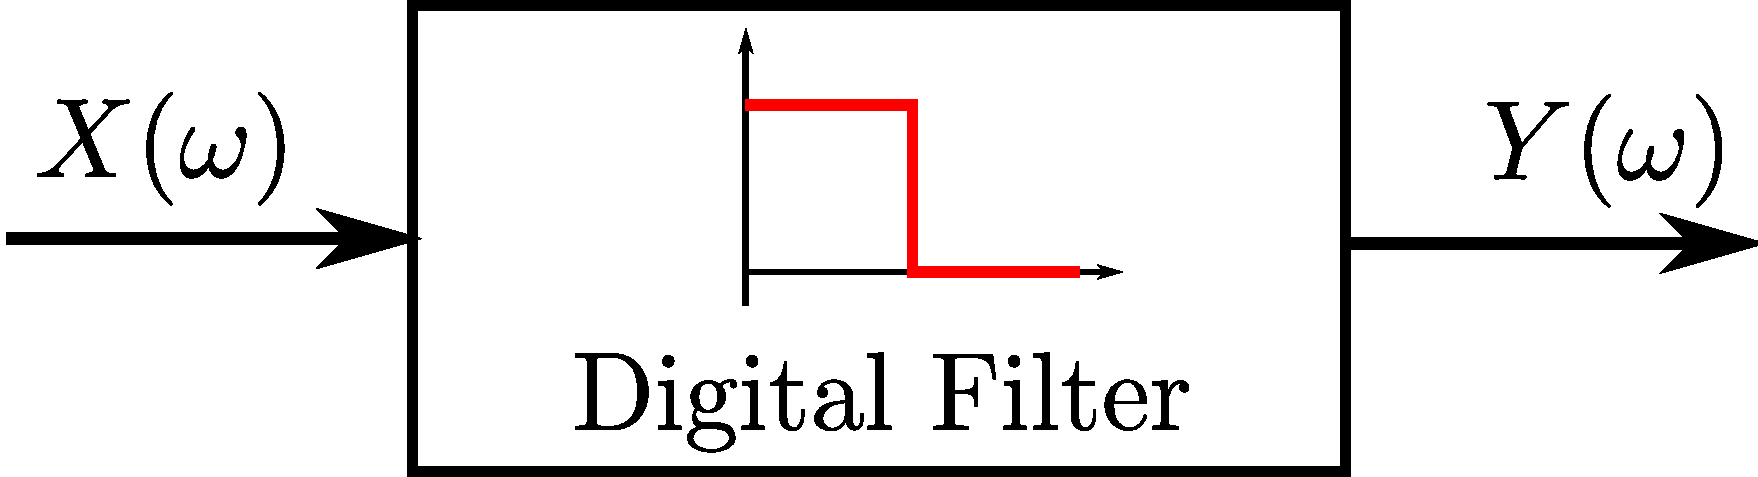
\includegraphics[width=0.7\textwidth]{JDD2014/figures/abstractFilterFrequency}
\end{figure}
$$Y(\omega)=\textcolor{blue}{H_d(\omega)}X(\omega),\omega\in[0,\pi]$$
Two types of filters:
\begin{itemize}
\small
\item finite impulse response (\textbf{FIR}) $\Rightarrow$ $H_d(\omega)$ \textbf{polynomial}
\item infinite impulse response (\textbf{IIR}) $\Rightarrow$ $H_d(\omega)$ \textbf{rational function}
\end{itemize}

\end{frame}

\begin{frame}
\frametitle{\textcolor{red}{AriC} -- Digital Filter Design}

FIR case:
$H_{d}(\omega)=\sum_{k=0}^{L}a_{k}\cos(\omega k)$
\vspace{0.1in}

\begin{columns}[c]

\column{2.6in}

\includegraphics<1-1>[width=1.0\textwidth]{JDD2014/figures/idealSpec}
\includegraphics<2-2>[width=1.0\textwidth]{JDD2014/figures/filterSpec}
\includegraphics<3-3>[width=1.0\textwidth]{JDD2014/figures/filterSpecWithOptim}
\includegraphics<4-4>[width=1.0\textwidth]{JDD2014/figures/filterSpecWithNaive}
\includegraphics<5->[width=1.0\textwidth]{JDD2014/figures/filterSpecFinal}

\column{2.3in}
Steps:
\vspace{0.05in}
\tiny

\uncover<3->{
1. Optimal filter computation:
\textcolor{red}{$$H_{d}(\omega)=\sum_{k=0}^{L}a_{k}\cos(\omega k)$$}}

\uncover<4->{
Naive rounding:
\textcolor{darkgreen}{$$\overline{H}_{d}(\omega)=\sum_{k=0}^{L}\overline{a}_{k}\cos(\omega k)$$}}

\uncover<5->{
2. Coefficient quantization:
\textcolor{blue}{$$H^{*}_{d}(\omega)=\sum_{k=0}^{L}a^{*}_{k}\cos(\omega k)$$}}

\normalsize

\end{columns}
\uncover<6->{Goal: filter synthesis toolchain for embedded and FPGA targets}
\end{frame}


%
% Partie Philippe
%

\begin{frame}<5>
  \frametitle{\textcolor{red}{AriC}}

  \tikzstyle{na} = [baseline=-.5ex]

  \begin{columns}
    \begin{column}{0.18\textwidth}
      \hspace*{-.7cm}\tikz[baseline]{
        \node[fill=red!10,anchor=base,text width=2.6cm, text centered]
        (n1) {\begin{tiny}
            \textbf{Exact}
            \hspace{1.5cm}
            Exact arithmetic
            \hspace{0.5cm}
            Computer algebra
            \hspace{2.2cm}
            \textbf{Approximate}
            \hspace{0.5cm}
            Floating-point arithmetic
            \hspace{1cm}
            Interval arithmetic
        \end{tiny}};}
    \end{column}

    \begin{column}{0.08\textwidth}
      \uncover<1-3>{\hspace*{-1cm}\tikz[baseline]{ \node[fill=white!30,anchor=base,text width=3cm, text centered,scale=1] (t1) {\color{red} {\footnotesize  Structured linear algebra } };}}

      \vspace{2cm}

      \uncover<1-4>{\tikz[baseline]{ \node[anchor=base, text centered,scale=1] (t2) {\color{red}{\footnotesize Lattices }}; }}


      \vspace{2cm}

      \uncover<1,4,5>{\hspace*{-1cm}\tikz[baseline]{ \node[fill=white!20,anchor=base,text width=2.8cm, text centered,scale=1] (t3) {\color{red}  {\footnotesize Numerical Linear Algebra}} ; }}

    \end{column}


    \column{0.2\textwidth}

    \uncover<1,2>{\hspace*{-1.2cm}\tikz[baseline]{\node[anchor=base,text width=1.5cm, text centered,scale=1] (t4) {\color{red} \begin{tiny}
          Polynomial
      \end{tiny}};}}

    \vspace*{0.1cm}

    \uncover<1,3,4>{\hspace*{-1.2cm}\tikz[baseline]{\node[ellipse,anchor=base,text width=1cm, text centered,scale=1] (t5) {\color{red} {\tiny Euclidean}};}}



    \column{0.3\textwidth}
    \uncover<1,2>{\hspace*{-1.5cm}\tikz[baseline]{\node[fill=white!30,anchor=base,text width=2cm, text centered,scale=1] (n2) {{\footnotesize Multivariate Interpolation}};}}

    \vspace*{1cm}

    \uncover<1,3>{\hspace*{-1.2cm}\tikz[baseline]{\node[fill=white!20,anchor=base,text width=3.5cm, text centered,scale=1] (n3) {{\footnotesize Learning With Errors structured version }};}}

    \vspace*{1.2cm}

    \uncover<1,4>{\hspace*{-1.5cm}\tikz[baseline]{\node[fill=white!20,anchor=base,text width=3cm, text centered,scale=1] (n4) {{\footnotesize Numerical functions and
    digital filters}};}}

    \vspace*{1cm}

    \uncover<1,5>{\hspace*{-1.5cm}\tikz[baseline]{\node[fill=white!20,anchor=base,text width=2.5cm, text centered,scale=1] (n5) {{\footnotesize Interval Linear Algebra}};}}
    %\end{column}



    \column{0.1\textwidth}
    \uncover<1,2>{\hspace*{-1.5cm}\tikz[baseline]{\node[fill=white!20,anchor=base,text width=3cm, text centered,scale=1] (m2) {{\scriptsize Applications to error-correcting codes}};}}

    \vspace*{1cm}

    \uncover<1,3>{\hspace*{-1.2cm}\tikz[baseline]{\node[fill=white!20,anchor=base,text width=2.5cm, text centered,scale=1] (m3) {{\scriptsize Cryptographic applications}};}}

    \vspace*{1cm}

    \uncover<1,4>{\hspace*{-1.5cm}\tikz[baseline]{\node[fill=white!20,anchor=base,text width=3cm, text centered,scale=1] (m4) {{\scriptsize FPGA Implementations}};}}

    \vspace*{1cm}

    \uncover<1,5>{\hspace*{-1.5cm}\tikz[baseline]{\node[fill=white!20,anchor=base,text width=3cm, text centered,scale=1] (m5) {{\scriptsize Certified parallel linear algebra library}};}}


  \end{columns}

  \begin{tikzpicture}[overlay]
    \uncover<1-3>{\path[black, thick,->] (n1) edge [out=80, in=180] (t1);}
    \uncover<1-4>{\path[black,thick,->] (n1) edge [out=0, in=180] (t2);}
    \uncover<1,4,5>{\path[black,thick,->] (n1) edge [out=-80, in=180] (t3);}
    \uncover<1,3>{\path[red!40,thick,->] (t5) edge [out=5, in=185] (n3);}
    \uncover<1,2>{\path[MyGreen!40,thick,->] (t4) edge [out=25, in=210] (n2);}
    \uncover<1,4>{\path[blue!50,thick,->] (t5) edge [out=0, in=175] (n4);}
    \uncover<1,4>{\path[blue!50,thick,->] (t3) edge [out=10, in=185] (n4);}
    \uncover<1,5>{\path[MyPurple!70,thick,->] (t3) edge [out=-5, in=175] (n5);}
    \uncover<1,2>{\path[MyGreen!40,thick,->] (t1) edge [out=5, in=190] (n2);}
    \uncover<1,3>{\path[red!40,thick,->] (t1) edge [out=-5, in=175] (n3);}
    \uncover<1,2>{\path[MyGreen!50,thick,->] (n2) edge [out=0, in=180] (m2);}
    \uncover<1,3>{\path[red!40,thick,->] (n3) edge [out=0, in=180] (m3);}
    \uncover<1,4>{\path[blue!50,thick,->] (n4) edge [out=0, in=180] (m4);}
    \uncover<1,5>{\path[MyPurple!70,thick,->] (n5) edge [out=0, in=180] (m5);}
    
    
  \end{tikzpicture}
\end{frame}

% \begin{frame}{Numerical Linear Algebra}
%   \[
%   \begin{pmatrix}
%     1.20 & 0.40 \\
%     8.00 & 2.50 
%   \end{pmatrix}
%   \begin{pmatrix}
%     44.3 & 2.10\cdot10^{+3} \\
%     12.6 & 2.60\cdot10^{-3}
%   \end{pmatrix}
%   \]
%   \[
%   \approx
%   \begin{pmatrix}
%     58.2 & 2.52\cdot10^{+3} \\
%     386 & 1.68\cdot10^{+4}
%   \end{pmatrix}
%   \]
% \end{frame}

% \begin{frame}{Numerical Interval Matrix Multiplication}
%   \[
%   \begin{pmatrix}
%     [1, 2] & [0,4] \\
%     [8, 8] & [2,3] 
%   \end{pmatrix}
%   \begin{pmatrix}
%     [44,45] & [2\cdot10^{+3}, 3\cdot10^{+3}] \\
%     [12,13] & [2\cdot10^{-3}, 3\cdot10^{-3}]
%   \end{pmatrix}
%   \]
%   \[
%   \subseteq
%   \begin{pmatrix}
%     [44,142]  & [2\cdot10^{+3},6\cdot10^{+3}] \\
%     [376,399] & [1.6\cdot10^{+4},2.4\cdot10^{+4}]
%   \end{pmatrix}
%   \]
% \end{frame}

% \begin{frame}{Classical 3-loops Algorithm}
%   \begin{spacing}{1.2}
%     \begin{algorithmic}[1]
%       \REQUIRE ${\bfm{A}} = [\ul A, \ol A]\in {\mathbb{I}}\mF^{m\times k},
%                {\bfm{B}} = [\ul B, \ol B]\in {\mathbb{I}}\mF^{k\times n}$
%       \ENSURE ${\bfm{C}} \in {\mathbb{I}}\mF^{m\times n},
%               {\bfm{C}} \supseteq {\bfm{A}} {\bfm{B}}$

%       \FOR{$i=1$ to $m$}
%       \FOR{$j=1$ to $n$}
%       \STATE $\ul C_{ij} \gets 0$; $\ol C_{ij} \gets 0$
%       \FOR{$l=1$ to $k$}
%       \STATE $\ul C_{ij} \gets \rounddown\left(\ul C_{ij} +
%         \min\left\{
%         \ul A_{il}\ul B_{lj}, \ul A_{il}\ol B_{lj},
%         \ol A_{il}\ul B_{lj}, \ol A_{il}\ol B_{lj}
%         \right\}\right)$
%       \STATE $\ol C_{ij} \gets \roundup\left(\ol C_{ij} +
%         \max\left\{
%         \ul A_{il}\ul B_{lj}, \ul A_{il}\ol B_{lj},
%         \ol A_{il}\ul B_{lj}, \ol A_{il}\ol B_{lj}
%         \right\}\right)$
%       \ENDFOR
%       \ENDFOR
%       \ENDFOR

%       \RETURN $[\ul C, \ol C]$
%     \end{algorithmic}
%   \end{spacing}
% \end{frame}

% \begin{frame}{Variant Interval Algorithms}
%   \begin{tabular}{lll}
%     Algorithm & Computed Radius & Cost 
%     \\
%     \texttt{MMMul3} &
%     at most $1.5\times$~exact radius &
%     about 3 \texttt{gemm}'s
%     \\
%     \texttt{MMMul5} &
%     at most $1.18\times$~exact radius &
%     about 5 \texttt{gemm}'s
%   \end{tabular}
% \end{frame}

% \begin{frame}{Criterion of Choice}
%   % Define block styles
%   \tikzstyle{decision} = [diamond, draw, fill=blue!20, 
%     text width=6em, text badly centered, inner sep=0pt]
%   \tikzstyle{block} = [rectangle, draw, fill=blue!20, 
%     text width=5em, text centered, rounded corners,
%     minimum height=2em]
%   \tikzstyle{line} = [draw, -latex']
%   \tikzstyle{cloud} = [draw, ellipse,fill=red!20,]

%   \begin{tikzpicture}[font=\small,node distance=2.5cm]
%     \node [block] (mul3) {\texttt{MMMul3}};
%     \node [block, right of=mul3] (mul2) {\texttt{MMMul2}};   
%     \node [block, left of=mul3] (mul5) {\texttt{MMMul5}};   
%     \node [decision, above of=mul3] (homogeneity)
%           {homegeneous precision?};
%     \node [decision, above of=mul5, node distance=4.5cm] (region2)
%           {medium precision?};
%     \node [cloud, above left of=region2, node distance=3.5cm] (e)
%           {Interval Matrix ${\bfm{A}}$};
%     \node [cloud, above right of=region2, node distance=3.5cm] (f)
%           {Interval Matrix ${\bfm{B}}$};
%     \path [line] (e) -- (region2);
%     \path [line] (f) -- (region2);
%     \path [line] (region2) -| node[near start,above]{no}  (homogeneity);
%     \path [line] (region2) -- node[near start,left]{yes} (mul5);
%     \path [line] (homogeneity)  -- node[near start,left]{no}  (mul3);
%     \path [line] (homogeneity) -|  node[near start,above]{yes} (mul2) ;
%   \end{tikzpicture}
% \end{frame}

% \begin{frame}{Parallel Implementation}
%   Problematic Rounding Mode Support:
%   \begin{itemize}
%   \item compiler
%   \item numerical library
%   \item multi-thread management
%   \end{itemize}
% \end{frame}

% fin partie Philippe


\begin{frame}<1>
  \frametitle{\textcolor{red}{AriC}}

  \tikzstyle{na} = [baseline=-.5ex]

  \begin{columns}
    \begin{column}{0.18\textwidth}
      \hspace*{-.7cm}\tikz[baseline]{
        \node[fill=red!10,anchor=base,text width=2.6cm, text centered]
        (n1) {\begin{tiny}
            \textbf{Exact}
            \hspace{1.5cm}
            Exact arithmetic
            \hspace{0.5cm}
            Computer algebra
            \hspace{2.2cm}
            \textbf{Approximate}
            \hspace{0.5cm}
            Floating-point arithmetic
            \hspace{1cm}
            Interval arithmetic
        \end{tiny}};}
    \end{column}

    \begin{column}{0.08\textwidth}
      \uncover<1-3>{\hspace*{-1cm}\tikz[baseline]{ \node[fill=white!30,anchor=base,text width=3cm, text centered,scale=1] (t1) {\color{red} {\footnotesize  Structured linear algebra } };}}

      \vspace{2cm}

      \uncover<1-4>{\tikz[baseline]{ \node[anchor=base, text centered,scale=1] (t2) {\color{red}{\footnotesize Lattices }}; }}


      \vspace{2cm}

      \uncover<1,4,5>{\hspace*{-1cm}\tikz[baseline]{ \node[fill=white!20,anchor=base,text width=2.8cm, text centered,scale=1] (t3) {\color{red}  {\footnotesize Numerical Linear Algebra}} ; }}

    \end{column}


    \column{0.2\textwidth}

    \uncover<1,2>{\hspace*{-1.2cm}\tikz[baseline]{\node[anchor=base,text width=1.5cm, text centered,scale=1] (t4) {\color{red} \begin{tiny}
          Polynomial
      \end{tiny}};}}

    \vspace*{0.1cm}

    \uncover<1,3,4>{\hspace*{-1.2cm}\tikz[baseline]{\node[ellipse,anchor=base,text width=1cm, text centered,scale=1] (t5) {\color{red} {\tiny Euclidean}};}}



    \column{0.3\textwidth}
    \uncover<1,2>{\hspace*{-1.5cm}\tikz[baseline]{\node[fill=white!30,anchor=base,text width=2cm, text centered,scale=1] (n2) {{\footnotesize Multivariate Interpolation }};}}

    \vspace*{1cm}

    \uncover<1,3>{\hspace*{-1.5cm}\tikz[baseline]{\node[fill=white!20,anchor=base,text width=3.5cm, text centered,scale=1] (n3) {{\footnotesize Learning With Errors structured version }};}}

    \vspace*{1.2cm}

    \uncover<1,4>{\hspace*{-1.5cm}\tikz[baseline]{\node[fill=white!20,anchor=base,text width=3cm, text centered,scale=1] (n4) {{\footnotesize Numerical functions and digital filters}};}}

    \vspace*{1cm}

    \uncover<1,5>{\hspace*{-1.5cm}\tikz[baseline]{\node[fill=white!20,anchor=base,text width=2.5cm, text centered,scale=1] (n5) {{\footnotesize Interval Linear Algebra}};}}
    %\end{column}



    \column{0.1\textwidth}
    \uncover<1,2>{\hspace*{-1.5cm}\tikz[baseline]{\node[fill=white!20,anchor=base,text width=3cm, text centered,scale=1] (m2) {{\scriptsize Applications to error-correcting codes}};}}

    \vspace*{1cm}

    \uncover<1,3>{\hspace*{-1.2cm}\tikz[baseline]{\node[fill=white!20,anchor=base,text width=2cm, text centered,scale=1] (m3) {{\scriptsize Cryptographic applications}};}}

    \vspace*{1cm}

    \uncover<1,4>{\hspace*{-1.5cm}\tikz[baseline]{\node[fill=white!20,anchor=base,text width=3cm, text centered,scale=1] (m4) {{\scriptsize FPGA Implementations}};}}

    \vspace*{1cm}

    \uncover<1,5>{\hspace*{-1.5cm}\tikz[baseline]{\node[fill=white!20,anchor=base,text width=3cm, text centered,scale=1] (m5) {{\scriptsize Certified parallel linear algebra library}};}}


  \end{columns}

  \begin{tikzpicture}[overlay]
    \uncover<1-3>{\path[black, thick,->] (n1) edge [out=80, in=180] (t1);}
    \uncover<1-4>{\path[black,thick,->] (n1) edge [out=0, in=180] (t2);}
    \uncover<1,4,5>{\path[black,thick,->] (n1) edge [out=-80, in=180] (t3);}
    \uncover<1,3>{\path[red!40,thick,->] (t5) edge [out=5, in=185] (n3);}
    \uncover<1,2>{\path[MyGreen!40,thick,->] (t4) edge [out=25, in=210] (n2);}
    \uncover<1,4>{\path[blue!50,thick,->] (t5) edge [out=0, in=175] (n4);}
    \uncover<1,4>{\path[blue!50,thick,->] (t3) edge [out=10, in=185] (n4);}
    \uncover<1,5>{\path[MyPurple!70,thick,->] (t3) edge [out=-5, in=175] (n5);}
    \uncover<1,2>{\path[MyGreen!40,thick,->] (t1) edge [out=5, in=190] (n2);}
    \uncover<1,3>{\path[red!40,thick,->] (t1) edge [out=-5, in=175] (n3);}
    \uncover<1,2>{\path[MyGreen!50,thick,->] (n2) edge [out=0, in=180] (m2);}
    \uncover<1,3>{\path[red!40,thick,->] (n3) edge [out=-10, in=180] (m3);}
    \uncover<1,4>{\path[blue!50,thick,->] (n4) edge [out=0, in=180] (m4);}
    \uncover<1,5>{\path[MyPurple!70,thick,->] (n5) edge [out=0, in=180] (m5);}
    
    
  \end{tikzpicture}
\end{frame}


\bibliographystyle{amsalpha}
\bibliography{biblio} 

\end{document}
